\documentclass[a4,10truept]{jsarticle}
\usepackage[top=24truemm,bottom=24truemm,left=22truemm,right=22truemm]{geometry}
\usepackage{graphicx}
\usepackage{bm}
\usepackage{wrapfig}
\usepackage{abstract}
\usepackage{cite}
\renewcommand{\baselinestretch}{1}
\renewcommand{\abstractname}{}
\renewcommand{\absnamepos}{empty}
\pagestyle{empty}
\usepackage{titlesec}
\titleformat*{\section}{\fontsize{12truept}{0truept} \bf \gt}

\begin{document}
\hspace{35truemm} \begin{minipage}{127truemm}
{\fontsize{14truept}{0truept} \selectfont \gt 金表面における中赤外プラズモンポラリトンの伝搬長測定\\ \rm Propagation length of mid-infrared surface plasmon\\ polaritons on gold\\ }\vspace{-0.8em}
{\fontsize{10truept}{0truept} \selectfont \mc \\ $^\bigcirc$平松信義$\!^{1,2)}$, 草史野$\!^{1,3)}$, 竹上明伸$\!^{1,3)}$, 今坂光太郎$\!^{1)}$, 森近一貴$\!^{1)}$, 芦原聡$\!^{1,\mathrm{a})}$\\ \rm Nobuyoshi Hiramatsu$^{1,2)}$, Fumiya Kusa$^{1,3)}$, Akinobu Takegami$^{1,3)}$, Kotaro Imasaka$^{1)}$, Ikki Morichika$^{1)}$, and Satoshi Ashihara$^{1,\mathrm{a})}$\\}
\end{minipage}\vspace{-0.5em}
{\mc \fontsize{10pt}{0pt} \selectfont \mc
東京大学生産技術研究所$\!^{1)}$, 東京大学物理工学科$\!^{2)}$, 東京農工大学物理システム工学専攻$\!^{3)}$\\ \rm
Institute of Industrial Science, the University of Tokyo$^{1)}$, Department of Applied Physics, the University of Tokyo$^{2)}$, Department of Applied Physics, Tokyo University of Agriculture and Technology$^{3)}$\\
email: ashihara@iis.u-tokyo.ac.jp$^{\mathrm{a})}$\\
}

\vspace{-0.9em}
\begin{abstract}
{\fontsize{10pt}{0pt} \rm We studied propagation length of surface plasmon polaritons (SPPs) at gold/air interface in the mid-infrared range. We showed that SPPs propagate for a distance of about or above $10\:\mathrm{mm}$ at a wavelength of $10.6\:\mathrm{\mu m}$, in good agreement with the value predicted from dielectric constant of polycrystalline gold. We also demonstrated that a simple treatment of thermal annealing led to noticeable elongation of SPP propagation length, accompanied by increased grain size and decreased surface roughness.}
\end{abstract}

\vspace{-1.4em}
\section{はじめに}
\vspace{-0.7em}
\mc 金属表面の中赤外プラズモニクスは, 物質に起因するロスが小さく高い電場増強度が達成できるため, 表面増強分光やバイオセンサ, プラズモニック回路への応用が可能である. 特に金は大気中で化学的に安定で, 導電率も高いことから, 優れたプラズモニック材料と言える. 本研究では金-空気界面を伝搬するプラズモンポラリトン(SPP)の伝搬長を, 波長$10.6\:\mathrm{\mu m}$(光源: $\mathrm{CO_2}\!$レーザー)において金のモルフォロジーと相関させて測定した. 

\vspace{-0.7em}
\section{デバイスと実験}
\vspace{-0.7em}
%\setlength{\intextsep}{0pt}
\setlength{\columnsep}{1em}%
\begin{wrapfigure}{R}[0mm]{0.35\hsize}
  \centering
  \raisebox{0pt}[\dimexpr\height-\baselineskip\relax]{\includegraphics[width=\hsize]{schematic.eps}}
    \caption{Schematic of the SPP waveguide devices.}
     \label{fig:schematic}
\end{wrapfigure}
SPPの伝搬長を測定するために, 図1に示すような一対の回折格子(入力/出力カップラー)と長さの異なるSPP導波路からなるデバイスの組を作成した. SPPは, まず自由空間伝搬光により入力カップラーで励起され, 導波路表面を伝搬し, 再び出力カップラーで伝搬光と結合する. ここで入力光と出力光のパワーの比は, 伝搬光とSPPの結合効率, SPPの伝搬効率(透過率), SPPと伝搬光の再結合効率の積で与えられ, 導波路の長さに依存して減衰する指数関数に従う. したがって入射光パワーとSPP-伝搬光結合効率を一定とすると, 各デバイスについて出力光のパワーを測定することにより伝搬長(SPPのパワーが1/eに落ち込む距離)が評価できる. 

入力/出力カップラー(溝深さ800 nm)と導波路(厚さ800 nm)の構造は, シリカ基板に蒸着された金下地(厚さ200 nm)の上に, さらに金の熱蒸着と電子線リソグラフィーを行うことで作成した. カップラーは表面リリーフ回折格子であり, 溝深さは厳密結合波解析法による計算で最適化した. 
金のモルフォロジーを制御するために試料は$600\:\mathrm{^\circ C}$ (20分)と$700\:\mathrm{^\circ C}$ (16分)で2段階アニール処理し, そのモルフォロジーを原子間力顕微鏡(AFM)と走査電子顕微鏡(SEM), 電子後方散乱回折法(EBSD)を用いて評価した.

\vspace{-0.7em}
\section{結果と考察}
\vspace{-0.7em}
導波路長さ$L$の関数である出力光パワーを, アニール前の試料(A), アニールを1回施した試料(B), アニールを2回施した試料(C)それぞれについて図2にプロットした. ここで出力光パワーは, それぞれの試料で指数フィッティングされており(実線), $L=0$の値をもとに正規化されている. 伝搬長さは試料A, B, Cに対してそれぞれ$9.0\pm0.3\:\mathrm{mm}$, $12.0\pm0.4\:\mathrm{mm}$, $14.7\pm0.7\:\mathrm{mm}$だった. アニールにより伝搬長が大きくなったことが見て取れる. この測定結果は金多結晶の誘電率\cite{Palik}による計算$12.3\:\mathrm{mm}$とよく一致した. 

\begin{wrapfigure}{r}[0mm]{0.4\hsize}
  \centering
\begin{minipage}{\hsize}
     \raisebox{0pt}[\dimexpr\height-\baselineskip\relax]{\includegraphics[width=0.9\hsize]{propagation_length.eps}}
    \caption{Semi-logarithmic plot of normalized output power as a function of the SPP waveguide length $L$}
       \label{fig:propagation_length}
\end{minipage}\\
\begin{minipage}{\hsize}
     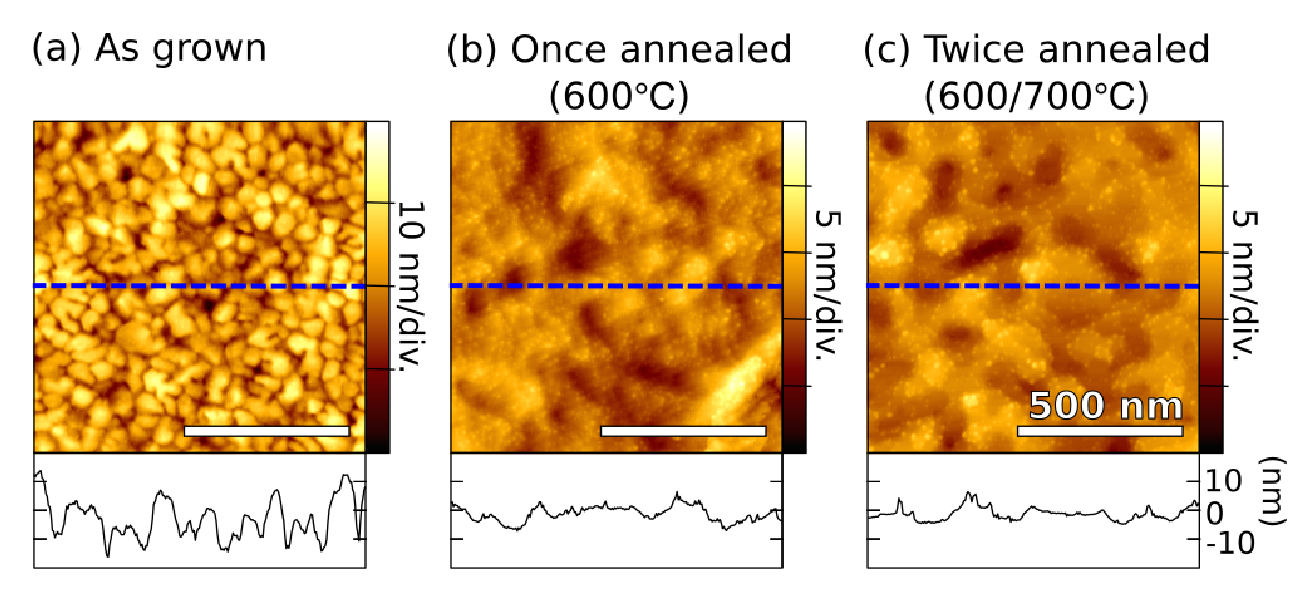
\includegraphics[width=\hsize]{morphology.eps}
        \caption{(a-c) AFM topographies and the corresponding cross sections, (d) SEM image, (e) EBSD pattern quality map, and (f) inverse pole figure: (a,b) correspond to the sample A,B, respectively, and (c-f) correspond to the sample C.}
    \label{fig:morphology}
\end{minipage}
\end{wrapfigure}
導波路表面でのAFMトポグラフィとその断面(トポグラフィ中の破線領域)を, 試料A,B,Cのそれぞれについて図3(a,b,c)に示した. 表面荒さは試料A, B, Cのそれぞれで5.7 nm, 2.8 nm, 2.2 nmであり, アニールにより表面荒さが小さくなったことがわかる. 図3(a)から試料Aについて, 多結晶に特有の結晶粒が明確に確認でき, その直径を$70\pm20\:\mathrm{nm}$と見積もった. 対して, アニール後の試料B,Cの結晶粒界はAFMトポグラフィからは不明瞭であり, 図3(d)に示す試料CのSEM写真でも同様に表面に明確な結晶粒界は見えない. そこで試料CについてEBSDによる結晶解析を行い, 図3(d)に対応する領域のパターンクオリティマップを図3(e)に示した. 白色の領域は高いパターンクオリティと結晶粒を意味し, 黒色の領域は結晶粒界や転移, 空孔に対応する. また図3(f)に薄膜法線方向に対する結晶方位の逆極点図を示した. 図3(e,f)から結晶粒の存在が確認でき, 図3(e)から結晶粒の大きさを$2000\pm1000\:\mathrm{nm}$と見積もった. アニールにより結晶粒が大きくなったことが見て取れる. 

本研究でアニールによりSPP伝搬長が大きくなったメカニズムを, 観測された結晶粒の増大と表面荒さの減少から考察する. Trollmannら\cite{Trollmann}が示したように, 結晶粒が大きくなると結晶粒界での自由電子の散乱レートとそれに起因するオームロスは小さくなる. またKuttgeら\cite{Kuttge}とLeeら\cite{Lee}らの報告によると, 伝搬するSPPの結晶粒界による散乱も損失に寄与する. したがって, 増大したSPP伝搬長は, 結晶粒が大きくなり結晶粒界の密度が小さくなったことと関連付けられる. それに対して, 表面荒さが小さくなるとオームロスは大きくなるため\cite{Trollmann}, 伝搬長の増大の説明には適さないと言える. また観測された表面荒さのSPPの散乱への影響は, 実験に用いた波長で極めて小さいと見積もれる\cite{Mills}. すなわち, 本研究で表面荒さの伝搬長への影響は無視できるか, 他の要因に比べ小さい. 我々は, アニールにより結晶粒界が大きくなったことが, SPP伝搬長が大きくなった大きな理由だと考える.

\vspace{-0.7em}
\section{結論}
\vspace{-0.7em}
金-空気界面を波長$10.6\:\mathrm{\mu m}$において伝搬するSPPの伝搬長が, 誘電率による計算とよく一致し, 10 mmを超えうることを実験で示した. また熱アニールの手続きによって伝搬長が大きくなると同時に, 結晶粒が大きく, 表面荒さが小さくなることを示した. 確認された伝搬長の増大は, アニールで結晶粒が大きくなったことにより, 結晶粒界でのオームロスとSPPの散乱が小さくなったことの影響であると我々は考える. SPPの伝搬長をモルフォロジーと関連付けて定量的に評価することは, プラズモニック導波路などの応用の観点のみならず, さらなるロスメカニズムの理解にも有用である. 

%\renewcommand{\refname}{}
%\bibliographystyle{unsrt}
%\bibliography{Reference}
\vspace{-0.7em}
\begin{thebibliography}{9}
\vspace{-0.7em}
\bibitem{Palik} E. D. Palik, "Handbook of Optical Constants of Solids," (Academic Press, 2002).
\bibitem{Trollmann} J. Trollmann and A. Pucci, J. Phys. Chem. C {\bf 118}, 15011 (2014).
\bibitem{Kuttge} M. Kuttge, E. J. R. Vesseur, J. Verhoeven, H. J. Lezec, H. A. Atwater, and A. Polman, Appl. Phys. Lett. {\bf 93}, 113110 (2008).
\bibitem{Lee} H. S. Lee, C. Awada, S. Boutami, F. Charra, L. Douillard, and R. E. de Lamaestre, Opt. Exp. {\bf 20}, 8974 (2012).
\bibitem{Mills} D. L. Mills, Phys. Rev. A {\bf 12}, 4036 (1975).
\end{thebibliography}

\end{document}